\subsection{Red McDonald's}

Para el siguiente experimento, capturamos los paquetes de la LAN Wi-Fi pública del McDonald's ubicado en el shopping Alto Avellaneda. La medición fue realizada un día sábado desde las 18 hs hasta las 20 hs. La cantidad de paquetes capturados es de aproximadamente 65.000. De todos estos, sólo 918 corresponden al protocolo ARP.

\begin{figure}[H]
       \centering
       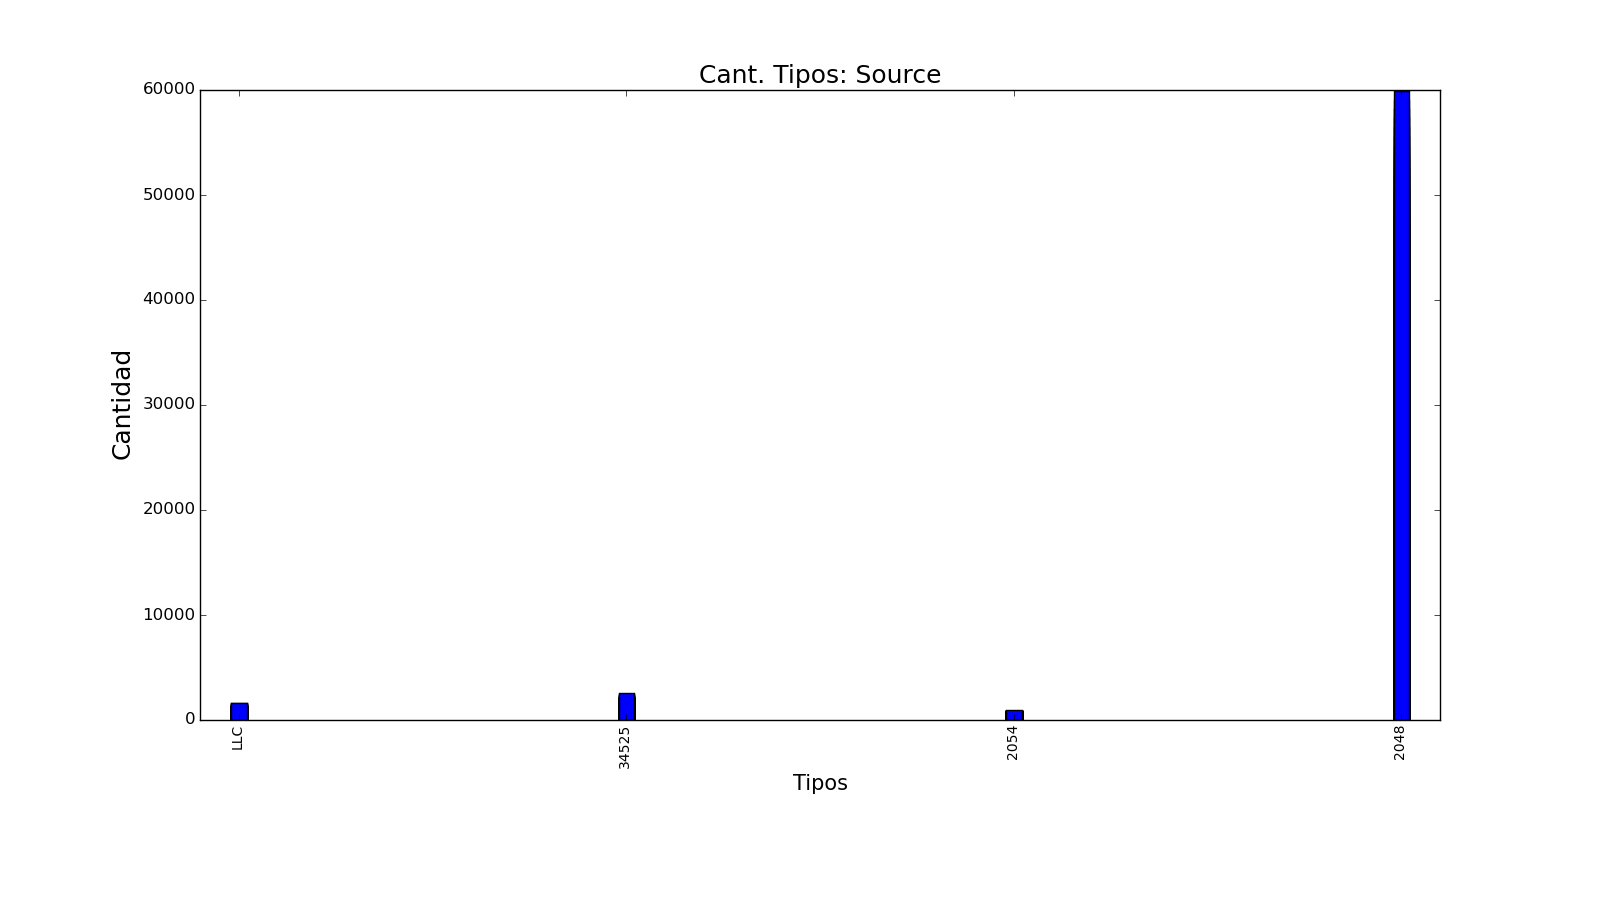
\includegraphics[width=1\textwidth]{../resultados/McDonalds/Basename_Source_hist}
       \caption{Protocolos de los paquetes capturados}
       \label{red-hogarena-types}
\end{figure}

